%%%%%%%%%%%%%%%%%%%%%%%%%%%%%%%%%%%%%%%%%%%%%%%%%%%%%%%%%%%%%%%%%%%%%%%%%%
%                                                      									 %
%                  		  	RPM Neutronic Performance   		            	 %
% 									                                                     %
%%%%%%%%%%%%%%%%%%%%%%%%%%%%%%%%%%%%%%%%%%%%%%%%%%%%%%%%%%%%%%%%%%%%%%%%%%
\section{RPM Neutronic Performance}
\label{sec:RPMNP}

Simulations are necessary to guide the design of a replacement RPM.
These simulations must provide a link between the measured performance of laboratory developed and characterized samples which are generally two inches and the performance of the film in an implemented detector system as it is prohibitive to construct and measure each film in an RPM.
Previous work showed that it is possible to adequately simulate detector performance in MCNPX, a Monte Carlo radiation transport code.
Generally these simulations involve correctly defining the simulation physics, source and geometry, and then using the correct tally measures to extract pertinent performance metrics.
After the simulation is completed is then benchmarked against measured quantities to provide a measure of confidence that the simulation provides an accurate model of reality.
Often (as in this case) the capability to directly measure the performance of the desired simulation geometry is not availabl is not available, and therefore the benchmarking must be completed on a comparable system on which it is possible to measure.

A validated simulation capability allows for one to explore the design space without having to physically build and test systems, which can be prohibitively expensive.
As a single film does not have the necessary interactions to fulfill the neutron count rate criteria multiple films are necessary, and the arrangement of these films provides a design space for a replacement RPM.
In the case of the RPM, there are several design parameters that can be explored:
\begin{itemize}
  \item the neutron absorber loading of the film,
  \item the thickness of the film,
  \item the geometry of the film (cylinders or sheets), and
  \item the placement of the films.
\end{itemize}
It is expected that the loading of the film will be limited by the optical clarity, and that the thickness of the film will be determined by the optimization of the energy deposition.
Thus, of the above design parameters only the geometric placement of the films is an available optimization space.

Preliminary work by this author provided a simple design in which the detector layers are linearly placed throughout the detector volume in an alternating fashion.
The analysis of the neutron flux throughout this detector lead to a flat flux profile as shown in \autoref{fig:AltLayerThermalNeutronFraction}.
\begin{figure}
  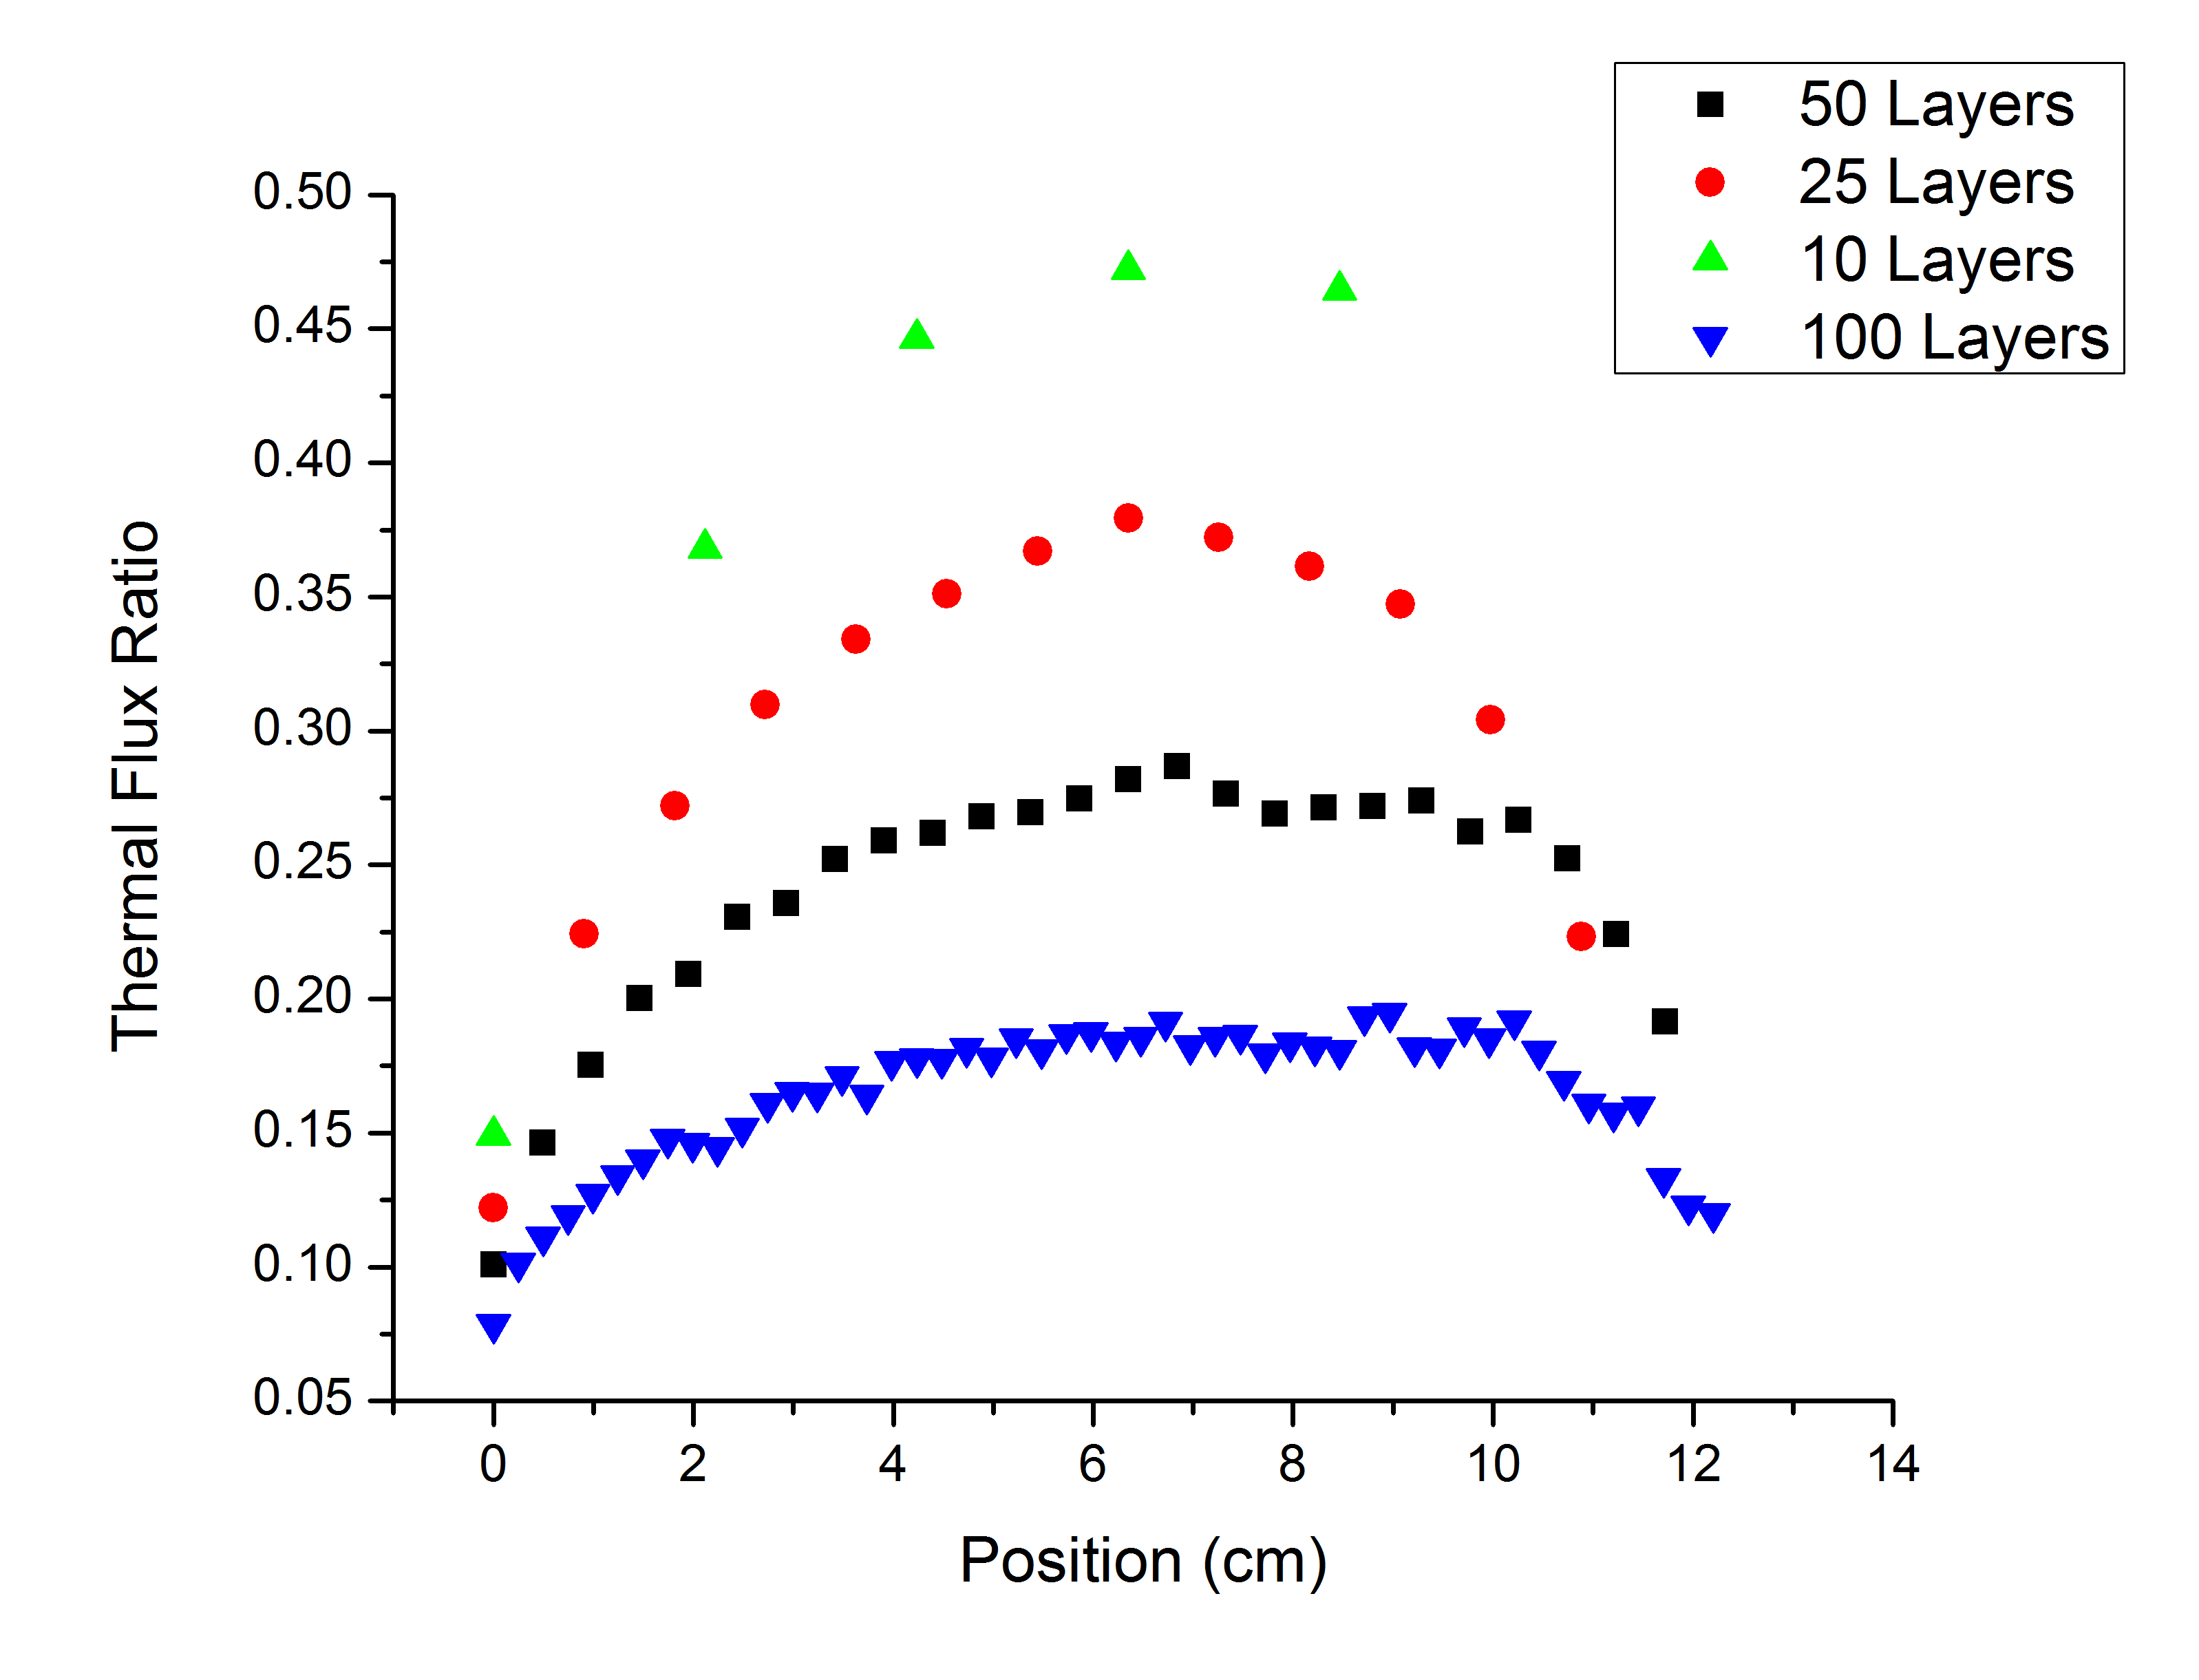
\includegraphics[width=\textwidth]{ThermalFluxRatioAltLayers}
	\caption{Fraction of the neutron flux that is thermalized through a alternating detector and moderator layered RPM.  The low thermal fluxes result in a poor utilization of the high thermal cross section of \iso[6]{Li}.}
	\label{fig:AltLayerThermalNeutronFraction}
\end{figure}
Several different strategies can then be used to optimize the geometry to ensure effective utilization of the thermal cross section of the absorber material.
\chapter{Summary, Deliverables and Timetable}
\label{ch:SummaryDeliverables}
\section{Summary}
Defense against nuclear terrorism relies upon the ability to accurately detect and identify Special Nuclear Material (SNM).
The current standard for neutron detection in portal monitors is \iso[3]{He}, which is a diminishing resource. 
A significant amount of research is then focused on developing new (or optimizing an existing) neutron detection system to serve as a replacement RPMs.
Previous work by this author focused on the characterization of replacement polymeric thin film detector technologies for RPMs.  
The proposed work will focus on designing a framework for determining an optimized detector design for replacement RPMs based on polymeric thin films.
This work will be novel in its utilization of high fidelity energy deposition to explain the origins of neutron-gamma discrimination through the range of secondary electrons from the neutron and photons reactions in their subsequent energy deposition.
The neutronic performance of a film will then be assessed by calculating the performance of a full scale replacement RPM in the test environment with MCNPX.
Non-linear search techniques will then be used to find the optimal geometry of the MCNPX model of the detector that best utilizes the neutron absorber.
Finally, the scintillation light from the detectors will be simulated with the GEANT4 toolkit, and the performance of the detector based upon the collected light signal reported.
Different light collection strategies will be employed to maximize the light collection efficiency and minimize the cost of electronics necessary for the detector.


\section{Delerivables and Timetable} 
The proposed optimization strategy will first optimize on the microscopic domain of the energy deposition of a single layered detector (supporting the simulations with measurements) and then optimize the performance on the macroscopic domain of a large area plastic scintillator detector.
What has been proposed is essentially an architecture for the optimization that can be broken down into modules.
For each of the subsystems, the developed code will be well documented in order to ensure that the toolkit is portable and with the ability to be extended.
In addition, self-contained repositories of the code base will be made available.
Doxygen, a standard tool for extracting documentation for annotated C++ sources will be used to develop HTML based documentation files and a project manual.
If time permits a tutorial will be developed to assist others in replicating this work.
Measurements made to validate the simulations will also be well documented, and hopefully self contained.
This is to ensure the portability of this work.
\autoref{fig:OptArc} is a flow chart of the proposed optimization process in which the energy deposition simulations influence the inputs of the neutronics modeling and the light transport simulations.
If either of these simulations indicate that the DHS/DNDO detector criteria will not be meet, it is then necessary to modify the detector thickness or material in order to design a detector that will meet the criteria. 
\begin{figure}
  \centering
  \includegraphics[width=0.75\textwidth]{optArch}
  \caption[Optimization Architecture]{Optimization Architecture.  The energy deposition module provides inputs into the MCNP neutronics model and the GEANT4 Light transport simulations. Parameters available for optimization are shown in yellow, while measurement feedback is shown in cyan.}
  \label{fig:OptArc}
\end{figure}

The timelines for the proposed work is presented in the following charts.
\autoref{fig:AdmTimeline} shows a broad overview of the project milestones and accomplishements.
In \autoref{fig:CompletedWorkTimeline} the energy deposition and neutronics optimization by genetic algothrims are shown.
Finally \autoref{fig:LightTransportTimeline} presents the timeline for simulation of light transport.
%%%%%%% ADMINISTRATIVE TIMELINE %%%%%
\begin{sidewaysfigure}
\begin{center}
\begin{ganttchart}[x unit=8.5mm,vgrid,time slot format=isodate,compress calendar,today=2013-08-05,today offset=.5,today label=Current Week,today rule/.style={draw=blue,ultra thick}]{2012-06-12}{2013-12-30}
\gantttitlecalendar{year} \\
\ganttgroup[progress=100]{Energy Modeling}{2012-06-15}{2013-06-01}\\
\ganttgroup[progress=90]{Neutronics Optimization}{2012-12-15}{2013-3-30}\\
\ganttgroup[progress=75]{GEANT4 Light Transport}{2013-4-1}{2013-9-1}\\
\ganttgroup[progress=50]{Write Up and Conclusions}{2013-7-1}{2013-10-1}\\
\ganttmilestone{Dissertation Proposal}{2013-8-9}\\
\ganttbar{Disserrtation Defense}{2013-10-1}{2013-11-1}\\
\ganttmilestone{Dissertation to Trace}{2013-11-27}\\
\ganttmilestone{Pass/Fail Form}{2013-11-27}\\
\end{ganttchart}
\end{center}
\caption{Proposed Adminstrative Timeline}
\label{fig:AdmTimeline}
\end{sidewaysfigure}
%%%%%%% COMPLETED WORK %%%%%%%
\begin{sidewaysfigure}
\begin{center}
\begin{ganttchart}[x unit=8.5mm,vgrid,time slot format=isodate,compress calendar,today=2013-08-05,today offset=.5,today label=Current Week,today rule/.style={draw=blue,ultra thick}]{2012-06-12}{2013-12-30}
\gantttitlecalendar{year} \\
\ganttgroup[progress=100]{Energy Modeling}{2012-06-15}{2013-06-01}\\
\ganttbar[progress=100]{Energy Deposition}{2012-06-15}{2013-4-15} \\
\ganttbar[progress=100]{Range}{2013-5-25}{2013-6-15} \\
\ganttmilestone{IEEE Secondary Electron Paper}{2013-06-15}\\
\ganttgroup[progress=90]{Neutronics Optimization}{2012-12-15}{2013-3-30}\\
\ganttbar[progress=100]{MCNP Neutronics}{2012-12-15}{2013-1-15} \\
\ganttbar[progress=100]{Scripted Input Decks}{2013-1-30}{2013-2-5}\\
\ganttlinkedbar[progress=90]{Genetic Algorthims}{2013-2-15}{2013-3-10}\\
\ganttmilestone{ANS Presentation}{2013-11-10}
\end{ganttchart}
\end{center}
\caption[Timeline of Completed Work]{Timeline of Completed Work.}
\label{fig:CompletedWorkTimeline}
\end{sidewaysfigure}
%%%% LIGHT TRANSPORT TIMELINE
\begin{sidewaysfigure}
\begin{center}
\begin{ganttchart}[x unit=8.5mm,vgrid,time slot format=isodate,compress calendar,today=2013-08-05,today offset=.5,today label=Current Week,today rule/.style={draw=blue,ultra thick}]{2012-06-12}{2013-12-30}
\gantttitlecalendar{year} \\
\ganttgroup[progress=75]{GEANT4 Validation}{2013-1-10}{2013-7-10}\\
\ganttbar[progress=100]{Flir Detectors}{2013-4-15}{2013-4-30}\\
\ganttbar[progress=100]{Fabrication of Detectors}{2013-1-10}{2013-7-10} \\
\ganttlinkedbar[progress=100]{GS20 Simulation}{2013-06-1}{2013-7-10}\\
\ganttlinkedbar[progress=80]{Layred Simulations}{2013-6-15}{2013-7-15}\\
\ganttgroup[progress=75]{GEANT4 RPM Light Transport}{2013-6-1}{2013-10-1}\\
\ganttbar[progress=50]{Prelimiary Simuation}{2013-7-1}{2013-7-20} \\
\ganttlinkedbar[progress=25]{Parameter Studies}{2013-8-1}{2013-9-1}\\
\ganttlinkedbar[progress=0]{Optimization}{2013-9-1}{2013-10-1}\\
\end{ganttchart}
\end{center}
\caption{Light Transport Timeline}
\label{fig:LightTransportTimeline}
\end{sidewaysfigure}
